\chapter{Bestimmung des optimalen Tunings \texorpdfstring{$k$}{k}} \label{cha:Optimierung}

Durch den Einfluss von viskoser Dämpfung ist die Absorberperformance
bei der Anregungsordnung $k_E$ nicht optimal, worauf in 
\secref{sec:Opt:SuboptDurchDaempfung} eingegangen wird.
%
Durch entsprechende Wahl des Absorbertunings kann die
bestmögliche Absorberwirkung dennoch bei der gewünschten Anregungsordnung erreicht werden.
Wie das Tuning zu wählen ist, wird in  \secref{sec:Opt:BedingungFuerMinimum} veranschaulicht.
Anschließend wird in  \secref{sec:Opt:Bsp}
die Anwendung der hergeleiteten Zusammenhänge an einem Beispiel demonstriert.

\section{Suboptimales Verhalten durch den Einfluss von Dämpfung}
\label{sec:Opt:SuboptDurchDaempfung}

Beim tautochronen Absorberentwurf nach \secref{subsec:TautDesignBedingungen} ist zunächst
keine Dämpfung berücksichtigt. 
Sollen Schwingungen mit Anregungsordnung $k_E$ vermieden werden, ist
die Wahl für das Absorbertuning $k=k_E$ sinnvoll (vgl. Guideline in \cite{Mayet:Tautochronic}).

Wird das Verhalten eines so ausgelegten Absorbers untersucht und dabei viskose Dämpfung berücksichtigt
(vgl. \secref{subsec:TautDesignNichtKonKrafte}), tritt ein unerwünschter Effekt auf.
Der Absorber zeigt nicht bei der Anregungsordnung $k_E$ die beste Performance,
sondern die beste Absorberwirkung verschiebt sich zu einer anderen Anregungsordnung $k_{E,shift}$. 
\figref{fig:Opt:Beispiel:Optimalesk1GanzerZoom} auf Seite \pageref{fig:Opt:Beispiel:Optimalesk1GanzerZoom} veranschaulicht diesen Effekt.
Das Minimum des Verlaufs, also der Punkt mit optimaler Absorberwirkung,  
des mit $k_1=k_E=1.5$ getunten Absorbers liegt nicht mehr bei $k_E = 1.5$, sondern
bei $k_{E,shift}\approx1.475$.
Je größer die  Dämpfung ist, desto ausgeprägter ist dieser Effekt.

Die Verschiebung der optimalen Absorberwirkung zu einer anderen Anregungsordnung $k_{E,shift}$
führt zwangsläufig zu einer Verschlechterung der Absorberperformance bei der
auftretenden Anregungsordnung $k_E$, bei welcher aber bestmögliche Performance vorliegen soll.
Durch die  Wahl des Absorbertunings $k$ kann dieser Verschlechterung unter Berücksichtigung 
der viskosen Dämpfung entgegengewirkt werden. 
Für $k\neq k_E$ findet eine Verschiebung des Verlaufs von $\vartheta$ über $k_E$ statt.
Dies kann dazu genutzt werden, um die Stelle bester
Absorberperformance durch optimale Wahl von $k=k_{opt}$ in Abhängigkeit der Dämpfung
auf die gewünschte Anregungsordnung $k_E$ zu verschieben.

Auf die Wahl des optimalen Tunings $k$ wird im Folgenden eingegangen.
Dabei wird eine analytische Optimalitätsbedingung hergeleitet, mit welcher das
optimale Tuning $k$ in Abhängigkeit der Anregungsordnung $k_E$ und der viskosen Dämpfung bestimmt
werden kann.




\section{Bedingung für Minimum von  \texorpdfstring{$\vartheta$}{vartheta}  an der Stelle \texorpdfstring{$k_E$}{kE}  }
\label{sec:Opt:BedingungFuerMinimum}


Im Rahmen dieser Herleitung von einer Periode $T = \frac{2\pi}{k_E}$ ausgegangen. Eine Erweiterung für
Systeme mit Periode  $T = \frac{2 \pi}{k_E} \lambda_L$ nach Gleichung \eqref{eq:DefinitionVonPeriodeUeberWelcheGeaveragedWird} 
mit $\lambda_L = \textsf{kgV} (\lambda_1, \lambda_2, \dots, \lambda_n)$ 
ist direkt möglich. 






\subsection{Herleitung der notwendigen Bedingung}

%
Um die Drehungleichförmigkeit $\vartheta$
%
nach \eqref{eq:DegreeOfIrregularity} für ein bestimmtes $k_E$ zu minimieren, muss das Integral  
\begin{equation}
	%\tilde{\vartheta} = 
	\frac{1}{T} \int_0^T{z^2 \dd \theta_{\psi}}
	\label{eq:OptDrehungleichfoermigkeitVereinfacht}
\end{equation}
minimal werden.
%
%
% Fourierentwicklungen
%
Für das weitere Vorgehen wird $z$, wie in \cite{Mayet:CPVAMitMistuning} vorgeschlagen,
durch eine Fourierreihe (vgl. \appref{ap:Fourierreihen:AllgDarstellung}) in der Form
\begin{equation}
	z = z_0 + \sum_{j=1}^{n_f} \left( a_j  \cos \left( j \frac{2 \pi}{T} \theta_{\psi} \right) + b_j  \sin \left( j \frac{2 \pi}{T} \theta_{\psi} \right) \right)
		\label{eq:OptFourierreiheFuerz}
\end{equation}
approximiert, wobei $n_f$ die Anzahl der Fourierkoeffizienten darstellt. 
Unter Verwendung von Gleichung \eqref{eq:OptFourierreiheFuerz} ergibt sich für das Integral über $z$ durch einfache Rechnung
%
%
%
%
% Integral über z
%
\begin{equation}
	\frac{1}{T} \int_0^T{z  \dd \theta_{\psi}} = 	z_0 = 0,
			\label{eq:OptFourierreiheIntegralUeberz}
\end{equation}
wobei das zweite Gleichheitszeichen für den hier betrachteten stationären Fall aus den
Averaging-Gleichungen \eqref{eq:AveragingGleichungenMitMistuningAblNachthetaTeil1vereinfacht} 
resultiert \cite{Mayet:CPVAMitMistuning}.  
Ähnliche Rechnung ergibt für Gleichung \eqref{eq:OptDrehungleichfoermigkeitVereinfacht}
%das hier auftretende Integral über $z^2$ 
den Zusammenhang
%
%
%
% Integral über z^2
%
\begin{equation}
	\frac{1}{T} \int_0^T{z^2  \dd \theta_{\psi}} = 	z_0^2 +  \sum_{j=1}^{n_f}{\left( \frac{a_j^2}{2} + \frac{b_j^2}{2} \right)} 
					= 	 \frac{1}{2} \sum_{j=1}^{n_f}{\left( a_j^2 + b_j^2 \right)} 
			\label{eq:OptFourierreiheIntegralUeberz2}
\end{equation}
%
%
%
% Zusammenhang von dz/dx mit allgemeinem x
%
und in analoger Weise resultiert mit Gleichung \eqref{eq:OptFourierreiheFuerz} allgemein (vgl. \cite{Mayet:CPVAMitMistuning})
%
\begin{equation}
	\frac{1}{T} \int_0^T{z \pdiff{z}{x} \dd \theta_{\psi}} = \frac{1}{2} \sum_{j=1}^{n_f}{\left(a_j \pdiff{a_j}{x} + b_j \pdiff{b_j}{x}\right)}.
				\label{eq:OptFourierreiheIntegralzdzdx}
\end{equation}















%
%
% Ableitung von zu minimierendem Integral nach k_E
%
Wichtiger Teil dieser Arbeit ist unter Verwendung der bestehenden Gleichungen eine
notwendige Bedingung für ein Minimum der Drehungleichförmigkeit $\vartheta$ an einer bestimmten Stelle $k_E$ herzuleiten.
Um eine notwendige Bedingung für ein Minimum vom Ausdruck \eqref{eq:OptDrehungleichfoermigkeitVereinfacht} 
%an einer bestimmten Stelle $k_E$ 
zu erhalten, wird die totale Ableitung nach $k_E$ gebildet.
Hierbei ist zu beachten, dass $a_j = a_j\left(\theta_{al} \left(k_E\right), I_{al}\left(k_E\right) \right)$ und $b_j = b_j\left(\theta_{al}\left(k_E\right), I_{al}\left(k_E\right) \right)$. Unter Berücksichtigung dieses Sachverhalts resultiert mit	\eqref{eq:OptFourierreiheIntegralUeberz2}
als notwendige Bedingung
%
\begin{equation}
	\begin{split}
	  & \frac{\dd}{\dd k_E}  \left(\frac{1}{T} \int_0^T{z^2 \dd \theta_{\psi}}\right) = \frac{\dd}{\dd k_E} \left( \frac{1}{2} \sum_{j=1}^{n_f}{\left[ a_j^2 + b_j^2\right]} \right) \\
	  & %= \frac{1}{2} \sum_{j=1}^{n_f} { \left[ \frac{\dd}{\dd k_E}  \left(a_j^2 + b_j^2\right) \right] } 
		  = \frac{1}{2} \sum_{j=1}^{n_f} { \left[ 2 a_j \frac{\dd a_j}{\dd k_E} + 2 b_j \frac{\dd b_j}{\dd k_E}\right] } \\
	  & = \sum_{j=1}^{n_f} { \left[      a_j \sum_{l=1}^{n} {\left( \pdiff{a_j}{{\theta_{al}}} \frac{\dd \theta_{al}}{\dd k_E} + \pdiff{a_j}{{I_{al}}} \frac{\dd I_{al}}{\dd k_E} \right) } 
	    + b_j \sum_{l=1}^{n} {\left( \pdiff{b_j}{{\theta_{al}}} \frac{\dd \theta_{al}}{\dd k_E} + \pdiff{b_j}{{I_{al}}} \frac{\dd I_{al}}{\dd k_E} \right) }  \right] } \\
		%	
		%& = \sum_{j=1}^{n_f} { \left[   \sum_{l=1}^{n} {\left( \left( a_j \pdiff{a_j}{{\theta_{al}}} + b_j  \pdiff{b_j}{{\theta_{al}}} \right) \frac{\dd \theta_{al}}{\dd k_E}  + \left( a_j \pdiff{a_j}{{I_{al}}}  + b_j \pdiff{b_j}{{I_{al}}} \right) \frac{\dd I_{al}}{\dd k_E}  \right) }  \right] }   \\
		%
		& = \sum_{l=1}^{n} { \left( \sum_{j=1}^{n_f}   {\left[ \left( a_j \pdiff{a_j}{{\theta_{al}}} + b_j  \pdiff{b_j}{{\theta_{al}}} \right) \frac{\dd \theta_{al}}{\dd k_E} 
		  + \left( a_j \pdiff{a_j}{{I_{al}}}  + b_j \pdiff{b_j}{{I_{al}}} \right) \frac{\dd I_{al}}{\dd k_E}  \right] }  \right) } 	\stackrel{!}= 0.
	\end{split}
	\label{eq:OptNotwBedUrsprForm}
\end{equation}
%
%
%
%
%
%
%
%
%
%%%%%%%%%%%%%%%%%%%%%%%%%%%%%%%%%%%%%%%%%%%%%%%%%%%%%%%%%%%%%%%%%%%%%%
% Bestimmung bestimmter Terme mit Hilfe der Averaging-Gleichungen
%%%%%%%%%%%%%%%%%%%%%%%%%%%%%%%%%%%%%%%%%%%%%%%%%%%%%%%%%%%%%%%%%%%%%
%
Nach Gleichung	\eqref{eq:OptFourierreiheIntegralzdzdx} gilt für die partiellen Ableitungen explizit
%
\begin{align}
	& \frac{1}{T} \int_0^T{z \pdiff{z}{{\theta_{al}}} \dd \theta_{\psi}} = \frac{1}{2} \sum_{j=1}^{n_f}{\left(a_j \pdiff{a_j}{{\theta_{al}}} + b_j \pdiff{b_j}{{\theta_{al}}}\right)} %= \frac{1}{2} \tilde{F}_{\theta_{al}}
	, \\
	%
	& \frac{1}{T} \int_0^T{z \pdiff{z}{{I_{al}}} \dd \theta_{\psi}} = \frac{1}{2} \sum_{j=1}^{n_f}{\left(a_j \pdiff{a_j}{{I_{al}}} + b_j \pdiff{b_j}{{I_{al}}}\right)} %= \frac{1}{2} \tilde{F}_{I_{al}}
	.
\end{align}
%
%
%
%
Durch Einsetzen in die Averaging-Gleichungen 
%
% Mistuning Gleichungen aus Averaging
%
\begin{align}
	& I_{al}^\prime = -\frac{\epsilon}{T} \int_0^T{z \pdiff{z}{{\theta_{al}}} \dd \theta_{\psi}} - \epsilon \delta_l I_{al} = 0, \\ 
	%
	& \theta_{al}^\prime = \frac{\epsilon}{T} \int_0^T{z \pdiff{z}{{I_{al}}} \dd \theta_{\psi}} + \frac{\epsilon}{T} \int_0^T{\pdiff{v}{{I_{al}}} \dd \theta_{\psi}} + \epsilon \bar{k}_l = 0 
\end{align}
nach \eqref{eq:AveragingGleichungenMitMistuningAblNachthetaTeil1vereinfacht}	 
und \eqref{eq:AveragingGleichungenMitMistuningAblNachthetaTeil2vereinfacht} resultieren die Zusammenhänge
%
%
%
% Mistuning Gleichungen aus Averaging mit Fourierentwicklung kombiniert
%
\begin{align}
	& \sum_{j=1}^{n_f}{\left(a_j \pdiff{a_j}{{\theta_{al}}} + b_j \pdiff{b_j}{{\theta_{al}}}\right)} = %- \frac{2}{T} \int_0^T{\pdiff{v}{{\theta_{al}}} \dd \theta_{\psi}} 
	- 2 \delta_l I_{al}
	\label{eq:OptAverGlIalUmgeschrieben}, \\
	%
	& \sum_{j=1}^{n_f}{\left(a_j \pdiff{a_j}{{I_{al}}} + b_j \pdiff{b_j}{{I_{al}}}\right)} = - \frac{2}{T} \int_0^T{\pdiff{v}{{I_{al}}} \dd \theta_{\psi}} - 2 \bar{k}_l
	\label{eq:OptAverGlThetaalUmgeschrieben},
\end{align}
%
%
%
%
mit welchen sich die notwendige Bedingung 	\eqref{eq:OptNotwBedUrsprForm}  zu
%
% Gesamte zu minimierende Gleichung
%
\begin{equation}
			\sum_{l=1}^{n} { \left(  \delta_l I_{al}  \frac{\dd \theta_{al}}{\dd k_E} 
		  + \left(  \frac{1}{T} \int_0^T{\pdiff{v}{{I_{al}}} \dd \theta_{\psi}} +  \bar{k}_l \right)  \frac{\dd I_{al}}{\dd k_E}    \right) } 	= 0
\end{equation}
ergibt.

%
%
% Definition der Abkürzungen für v-Terme
%
Mit der abkürzenden Schreibweise
\begin{equation}
		%\tilde{V}_{\theta_{al}} =  \frac{1}{T} \int_0^T{\pdiff{v}{{\theta_{al}}} \dd \theta_{\psi}},     \qquad       
		\tilde{V}_{I_{al}} = \frac{1}{T} \int_0^T{\pdiff{v}{{I_{al}}} \dd \theta_{\psi}}
		\label{eq:OptAbkuerzungVonVTerm}
\end{equation}
%
%
lautet die Bedingung in kompakter Form
%
% Gesamtgleichung mit Abkürzungen
% 
\begin{equation}
			\sum_{l=1}^{n} { \left(   \delta_l I_{al}  \frac{\dd \theta_{al}}{\dd k_E} 
		  + \left( \tilde{V}_{I_{al}}  +  \bar{k}_l \right)  \frac{\dd I_{al}}{\dd k_E}    \right) } 	= 0.
			\label{eq:OptMinimumsbedingungKompakt}
\end{equation}
%
Die hier auftretenden Gradienten $\frac{\dd \theta_{al}}{\dd k_E}$ und $\frac{\dd I_{al}}{\dd k_E}$ werden im folgenden Abschnitt bestimmt.























\subsection{Bestimmung der Gradienten} \label{Opt:Theorie:BestDerGrad}
%
%
%
Die Gleichungen 	\eqref{eq:OptAverGlIalUmgeschrieben} und 	\eqref{eq:OptAverGlThetaalUmgeschrieben} lauten mit
den Abkürzungen
%
% Abkürzungen tilde{F}-Terme
%
\begin{equation}
		\tilde{F}_{\theta_{al}} =  \sum_{j=1}^{n_f}{\left(a_j \pdiff{a_j}{{\theta_{al}}} + b_j \pdiff{b_j}{{\theta_{al}}}\right)} ,     \qquad  
		\tilde{F}_{I_{al}} =  \sum_{j=1}^{n_f}{\left(a_j \pdiff{a_j}{{I_{al}}} + b_j \pdiff{b_j}{{I_{al}}}\right)}
		\label{eq:Opt:BestDerGrad:FTildeTerme}
\end{equation}
%
%
%
und mit Gleichung \eqref{eq:OptAbkuerzungVonVTerm} in kompakter Schreibweise
%
\begin{align}
	& \tilde{F}_{\theta_{al}}  + 2 \delta_l I_{al} = 0, \\
	%
	& \tilde{F}_{I_{al}} + 2 \tilde{V}_{I_{al}} + 2 \bar{k}_l = 0.
\end{align}
%
%
%
%
% Ableitung der beiden Gleichungen
%
Ableiten der beiden Gleichungen nach $k_E$ ergibt
\begin{equation}
	\frac{\dd}{\dd k_E}   \left(  \tilde{F}_{\theta_{al}}  + 2 \delta_l I_{al}    \right)   
	= \pdiff{\tilde{F}_{\theta_{al}}}{{\theta_{al}}}  \frac{\dd \theta_{al}}{\dd k_E} +  \pdiff{\tilde{F}_{\theta_{al}}}{{I_{al}}}    \frac{\dd I_{al}}{\dd k_E} 
	   + 2 \delta_l \frac{\dd I_{al}}{\dd k_E}  = 0 
\end{equation}
%
und
%
\begin{equation}
	\begin{split}
	& \frac{\dd}{\dd k_E}   \left(\tilde{F}_{I_{al}} + 2 \tilde{V}_{I_{al}} + 2 \bar{k}_l \right)  \\
	& = \pdiff{\tilde{F}_{I_{al}}}{{\theta_{al}}}  \frac{\dd \theta_{al}}{\dd k_E} +  \pdiff{\tilde{F}_{I_{al}}}{{I_{al}}}    \frac{\dd I_{al}}{\dd k_E} 
	  + 2 \pdiff{\tilde{V}_{I_{al}}}{{\theta_{al}}}  \frac{\dd \theta_{al}}{\dd k_E} + 2 \pdiff{\tilde{V}_{I_{al}}}{{I_{al}}}    \frac{\dd I_{al}}{\dd k_E}  + 2 \frac{\dd \bar{k}_l}{\dd k_E}  = 0,  
	\end{split}
\end{equation}
%
%
%
%
%
% Matrixscheibweise
%
was in Matrixschreibweise $\vA \vx = \vb$ zu
\begin{equation}
	\bmat{ \pdiff{\tilde{F}_{I_{al}}}{{\theta_{al}}} + 2 \pdiff{\tilde{V}_{I_{al}}}{{\theta_{al}}}  & \pdiff{\tilde{F}_{I_{al}}}{{I_{al}}} + 2 \pdiff{\tilde{V}_{I_{al}}}{{I_{al}}}   \cr 
	       \pdiff{\tilde{F}_{\theta_{al}}}{{\theta_{al}}} 								 & \pdiff{\tilde{F}_{\theta_{al}}}{{I_{al}}}  + 2 \delta_l }
	\bmat{\frac{\dd \theta_{al}}{\dd k_E} \cr \frac{\dd I_{al}}{\dd k_E}}
	= \bmat{-2 \frac{\dd \bar{k}_l}{\dd k_E}  \cr 0  			\rule[-\dp\strutbox]{0pt}{ \totalheightof{$\frac{\dd\bar{k}_l}{\dd k_E}$}  } }
	\label{eq:OptGradInMatrix}
\end{equation}
%
zusammengefasst wird.
%
%
% abkürzende Schreibweise zum invertieren Ax = b
%
Mit dem allgemeinen Zusammenhang 
\begin{equation}
	\bmat{a_{11} & a_{12}  \cr a_{21} & a_{22}  } \bmat{x_1 \cr x_2} = \bmat{b_1 \cr 0} \quad
	%
	\Rightarrow \quad  
	\bmat{x_1 \cr x_2} %= \bmat{a_{11} & a_{12}  \cr a_{21} & a_{22} }^{-1}  \bmat{b_1 \cr 0} 
	= \frac{1}{\det(\vA)}  \bmat{a_{22} & -a_{12}  \cr -a_{21} & a_{11} } \bmat{b_1 \cr 0}
	= \frac{b_1}{\det(\vA)}  \bmat{a_{22} \cr -a_{21}}
\end{equation}
für ein $2\times2$-System der Form $\vA \vx = \vb$ mit $\det(\vA) = a_{11}a_{22} - a_{12}a_{21} \neq 0$ ergibt sich für das 
in Gleichung \eqref{eq:OptGradInMatrix} betrachtete
System 
%
%
%
%
%
\begin{equation}
	\bmat{\frac{\dd \theta_{al}}{\dd k_E} \\[2pt] \frac{\dd I_{al}}{\dd k_E}} 
	= 	-2 \frac{\dd \bar{k}_l}{\dd k_E}		\left( \det(\vA) \right) ^{-1}     
			\bmat{   \pdiff{\tilde{F}_{\theta_{al}}}{{I_{al}}}  + 2 \delta_l      \\[2pt]   
			- \pdiff{\tilde{F}_{\theta_{al}}}{{\theta_{al}}} }.
\end{equation}
%
%
%
Damit resultiert für die Minimumsbedingung 	\eqref{eq:OptMinimumsbedingungKompakt} zur
Bestimmung des optimalen Tunings $k_{l,opt}$ endgültig
%
\begin{equation}
			\sum_{l=1}^{n} { \left(   \delta_l I_{al}   \left(  \pdiff{\tilde{F}_{\theta_{al}}}{{I_{al}}}  + 2 \delta_l  \right)
		                  - \left( \tilde{V}_{I_{al}}  +  \bar{k}_l \right)    \pdiff{\tilde{F}_{\theta_{al}}}{{\theta_{al}}}    \right) } 	= 0.
			\label{eq:OptMinimumsbedinungEndg}								
\end{equation}
%
%
%
Bei Gleichung \eqref{eq:OptMinimumsbedinungEndg} handelt es sich um eine notwendige Bedingung für ein Minimum
bzw.  für ein Extremum. 
Ist \eqref{eq:OptMinimumsbedinungEndg}  erfüllt, muss es sich nicht zwangsweise um ein Minimum handeln, sondern
es könnte theoretisch auch ein Maximum oder ein Sattelpunkt vorliegen.
Um sicher zu stellen, dass es sich definitiv um
ein Minimum handelt, müsste zusätzlich noch die zweite Ableitung betrachtet werden.
%
Da bekannt ist, dass $k_{l,opt}\approx k_E$ für mäßige Dämpfung gilt, kann 
%Da diese Berechnung sehr aufwendig ist, wird 
im Rahmen dieser Arbeit darauf verzichtet werden. 
%
Ist Gleichung	\eqref{eq:OptMinimumsbedinungEndg} erfüllt bzw. hat sie sogar mehrere Lösungen,
ist es dennoch sinnvoll zu prüfen, ob es sich bei diesen um ein Minimum handelt.
 %müssen die potentiellen Lösungen noch darauf überprüft werden,
%ob es sich bei diesen um ein Minimum handelt.
Dies kann beispielsweise durch Betrachtung des resultierenden Verlaufs von $\vartheta$ über $k_E$ erfolgen
und wird im folgenden Abschnitt anhand eines Beispiels veranschaulicht.



\section{Beispiel für einen Absorber}
\label{sec:Opt:Bsp}

Nun wird die im vorigen Abschnitt hergeleitete Minimumsbedingung beispielhaft 
für die Berechnung des optimalen Tunings $k_{1,opt}$ eines Absorbers angewendet.
Dabei werden die resultierenden Gleichungen explizit angegeben und die daraus abgeleiteten Ergebnisse veranschaulicht.
Zudem wird aufgezeigt, was für Probleme auftreten können und wie diese beispielsweise durch 
sinnvolle Wahl der Startwerte bei der Optimierung vermieden werden können.


\subsection{Averaging-Gleichungen} \label{Opt:Bsp:AveragingGleichungen}
%
%
%
%
Nach \eqref{eq:AveragingGleichungenMitMistuningAblNachthetaTeil1vereinfacht} und 
\eqref{eq:AveragingGleichungenMitMistuningAblNachthetaTeil2vereinfacht} lauten die Averaging-Gleichungen
für einen Absorber  
%
%
%
% Vereinfachte Averaging-Gleichungen
%
\begin{align}
		& \tilde{\theta}_{a \psi}^\prime = \frac{\epsilon}{T} \int_0^T   z \dd \theta_{\psi},  &  
		& \theta_{a1}^\prime = \frac{\epsilon}{T} \int_0^T   \left(  z F_{I_{a1}} + V_{I_{a1}} \right)  \dd \theta_{\psi}        + \epsilon \bar{k}_1,  	\label{eq:OptBspEinAbsTeil1}\\
		& I_{a \psi}^\prime = 0, &
		& I_{a1}^\prime = - \frac{\epsilon}{T} \int_0^T  z F_{\theta_{a1}}  \dd \theta_{\psi}        - \epsilon \delta_1 I_{a1} .
	\label{eq:OptBspEinAbsTeil2}
\end{align}
%
%
%
Die in $z$ nach Gleichung \eqref{eq:HamiltonfunktionNachAveragingDefinitionVonz} benötigte  Funktion $f_1=f_1(s_1)$ wird durch
\begin{equation}
	f_1(s_1) = b_0 + b_2 s_1^2
	\label{eq:Opt:Bsp:Funktionf1}
\end{equation}
approximiert (vgl. \appref{ap:Rotationspendel} und \cite{Mayet:Tautochronic}) und das in $v$ nach Gleichung \eqref{eq:HamiltonfunktionNachAveragingMitMistuningDefVonv} 
auftretende nichtlineare Mistuning $u_1=u_1(s_1)$ wird als
\begin{equation}
	u_1(s_1) = u_{1,2} s_1^2 
	\label{eq:Opt:Bsp:MistAnsatz2terOrdn}
\end{equation}
mit $u_{1,2} \in \MR$ angesetzt (vgl. \chref{cha:UntersuchungenMistuning}).
Eine Erweiterung um beispielsweise Terme vierter Ordnung in $s_1$ in den Funktionen $f_1$ und $u_1$ ist in die Implementierung mit aufgenommen.
Außerdem ist der  Zusammenhang für $s_1$ nach 
Gleichung 	\eqref{eq:HamiltonAmplitudeSzuWinkelvariablen} zu berücksichtigen.



Mittelung über die Periode $T = \frac{2\pi}{k_E}$ ergibt die triviale Gleichung
\begin{equation}
	\tilde{\theta}_{a \psi}^\prime = \epsilon \left(c_0 + I_{a\psi} \right) = 0,
\end{equation}
%
%
%
%
sowie die das stationäre Verhalten beschreibenden Gleichungen
%
\begin{equation}
	\begin{split}
	\theta_{a1}^\prime &= k_1 - k_E + \epsilon I_{a1} u_{1,2} + \frac{\epsilon}{8  k_1}   \left( 6 I_{a1}^2  b_2^2 + 4 I_{a1} k_1^3 + 4  b_0^2 k_1^2 + 8 I_{a1}  b_0  b_2 k_1 \right)   \\
							&  -   \frac{\epsilon }{4 \sqrt{2 k_1 I_{a1}  } }   \left( 2 b_0 k_1 + 3 I_{a1} b_2  \right)   \Gamma   \sin(\theta_{a1})  = 0
	\end{split}
	\label{eq:OptBspGleichungThetaa1}
\end{equation}
%
und
%
\begin{equation}
	I_{a1}^\prime = \frac{\epsilon  \Gamma }{4 k_1} \sqrt{2 k_1 I_{a1}} \left( I_{a1} b_2 + 2 b_0 k_1 \right)  \cos(\theta_{a1}) 
	- \epsilon I_{a1}  \delta_1  = 0.
		\label{eq:OptBspGleichungIa1}
\end{equation}
%
%
Die Gleichungen \eqref{eq:OptBspGleichungThetaa1} 	und	\eqref{eq:OptBspGleichungIa1} entsprechen bis auf den Zusatzterm aufgrund des Mistuning-Ansatzes 
den in \cite{Mayet:Tautochronic} angegebenen Gleichungen für einen tautochronen Absorber.
Zu beachten ist jedoch, dass der Koeffizient $b_2$ indirekt durch das nichtlineare Mistuning beeinflusst wird.
Für die Drehungleichförmigkeit $\vartheta$ resultiert
\begin{equation}
	\begin{split}
	\vartheta  &= \frac{1}{\sqrt{2 k_1}}   \Bigg[   \Gamma^2 k_1 + I_{a1}^3 b_2^2 + I_{a1}^2 k_1^3 + 2 I_{a1} b_0^2 k_1^2 + 2 I_{a1}^2 b_0 b_2 k_1  \\
						 & \quad-  \sqrt{2 k_1 I_{a1}}  \Gamma  \sin(\theta_{a1})  \left( 2 b_0 k_1  +   I_{a1} b_2 \right)    \Bigg] ^{\frac{1}{2}} .
	\end{split}
	\label{Opt:Bsp:Vartheta}
\end{equation}
















\subsection{Bedingung für Minimum} \label{subsec:Opt:Bsp:BedFuerMinimum}
%
%
%
Die notwendige Bedingung für ein Minimum an der Stelle $k_E$ lautet nach Gleichung \eqref{eq:OptMinimumsbedinungEndg}	für einen Absorber
%
% Minimumsbedingung 1 Absorber
%
\begin{equation}
			 \delta_1 I_{a1}  \left( \pdiff{\tilde{F}_{\theta_{a1}}}{{I_{a1}}} + 2 \delta_1 \right)
		                  - \left( \tilde{V}_{I_{a1}} + \bar{k}_1 \right)  \pdiff{\tilde{F}_{\theta_{a1}}}{{\theta_{a1}}}   = 0
											\label{eq:OptBspMinimum1Abs}
\end{equation}
%
mit $\bar{k}_1 = \frac{k_1 - k_E}{\epsilon}$ nach Gleichung  \eqref{eq:AveragingNotwendigeBedingung}. Mit dem Ansatz für $u_1$ resultiert 
explizit
%
% Integral über dv/dI_a_1
%
\begin{equation}
	  \tilde{V}_{I_{a1}} = \frac{1}{T} \int_0^T{\pdiff{v}{{I_{a1}}} \dd \theta_{\psi}} = I_{a1} u_{1,2}. 
\end{equation}
%
%
%
%
%
%
Um die Terme $\pdiff{\tilde{F}_{\theta_{a1}}}{{I_{a1}}}$ und $\pdiff{\tilde{F}_{\theta_{a1}}}{{\theta_{a1}}}$  in \eqref{eq:OptBspMinimum1Abs} zu bestimmen,
müssen die Fourierkoeffizienten explizit berechnet werden, was in \appref{ap:Fourierreihen:1Absorber} dargestellt ist. Nach längerer Rechnung resultieren die Zusammenhänge
%
%
% Terme aus Fourierreihe
%
\begin{align}
		& \pdiff{\tilde{F}_{\theta_{a1}}}{{I_{a1}}}  
					%= - \frac{\sqrt{2} \Gamma \cos(\theta_{a1})  \left(3 I_{a1} b_2 + 2 b_0 k_1\right)}{4 \sqrt{k_1 I_{a1}} }
					%
					= - \frac{\Gamma} {2} \frac{1}{\sqrt{2 k_1 I_{a1}} }  \cos(\theta_{a1})  \left(3 I_{a1} b_2 + 2 b_0 k_1\right) 
					, \\
		%			
		& \pdiff{\tilde{F}_{\theta_{a1}}}{{\theta_{a1}}}  	
					%= \frac{\sqrt{2 I_{a1}} \Gamma  \sin (\theta_{a1})  \left(I_{a1} b_2 + 2 b_0 k_1\right)}{2 \sqrt{k_1}}
					%
					= \frac{\Gamma}{2} \sqrt{  \frac{2 I_{a1}}{k_1} } \sin (\theta_{a1})  \left(I_{a1} b_2 + 2 b_0 k_1\right)
					,
\end{align}
%
%
womit sich die notwendige Bedingung für eine Minimum des Verlaufs der Drehungleichförmigkeit $\vartheta$ über $k_E$ an einer bestimmten Stelle $k_E$ zu
%
% Minimumsbedingung 1 Absorber endgültig
%
\begin{equation}
	\begin{split}
			 & \delta_1 I_{a1}  \left( - \frac{\Gamma} {2} \frac{1}{\sqrt{2 k_1 I_{a1}} }  \cos(\theta_{a1})  \left(3 I_{a1} b_2 + 2 b_0 k_1\right)       + 2 \delta_1 \right)   \\
		   & - \left( I_{a1} u_{1,2} + \frac{k_1 - k_E}{\epsilon} \right)  \frac{\Gamma}{2} \sqrt{  \frac{2 I_{a1}}{k_1} } \sin (\theta_{a1})  \left(I_{a1} b_2 + 2 b_0 k_1\right) 
								= 0
	\end{split}
	\label{eq:OptBspMinimum1AbsEndg}
\end{equation}
%
ergibt. Somit stehen alle das Optimierungsproblem beschreibenden Gleichungen zur Verfügung.
%
Ziel ist es nun $\vartheta$ nach Gleichung	\eqref{Opt:Bsp:Vartheta} durch geeignete Wahl 
von $k_1=k_{1,opt}$  an einer bestimmten Stelle $k_E$ zu minimieren,
was durch Erfüllen der Minimumsbedingung \eqref{eq:OptBspMinimum1AbsEndg} erreicht wird.
Um das zu Grunde liegende mechanische Systemverhalten zu berücksichtigen, müssen bei der Minimierung von $\vartheta$ die das
Systemverhalten beschreibenden Averaging-Gleichungen	\eqref{eq:OptBspGleichungThetaa1} und \eqref{eq:OptBspGleichungIa1}  erfüllt sein.
%
% Die Gleichungen  \eqref{eq:OptBspGleichungThetaa1}, \eqref{eq:OptBspGleichungIa1} und \eqref{eq:OptBspMinimum1AbsEndg} stellen formal formal drei nichtlineare Nebenbedinungen im Optimierungsproblem von $\vartheta$ an einer bestimmen Stelle $k_E$  dar.










\newpage
\subsection{Lösung des Optimierungsproblems mit Matlab}

Das im vorherigen Abschnitt beschriebene Optimierungsproblem wird mit Hilfe der Funktion \texttt{fmincon},  
welche die Minimierung einer Zielfunktion $\vartheta$ mit Nebenbedingungen %beliebiger Form 
erlaubt,  in \textsc{Matlab} gelöst. 
Zunächst handelt es sich um ein Optimierungsproblem in der Form, 
dass die Zielfunktion $\vartheta$ durch Wahl von $k_1$  an einer bestimmen Stelle $k_E$ minimal werden soll (z.\,B. bei $k_E = 1.5$).
%
Zugleich soll der Verlauf der Zielfunktion $\vartheta$ über $k_E$ sein Minimum an dieser bestimmten Stelle $k_E$ annehmen, 
was durch Erfüllen der Minimumsbedingung \eqref{eq:OptBspMinimum1AbsEndg} in Form einer Gleichungsnebenbedingung erreicht wird.


Da die systembeschreibenden Averaging-Gleichungen $\theta_{a1}^\prime = 0$ und $I_{a1}^\prime=0$ nicht analytisch nach $\theta_{a1}$ und $I_{a1}$ aufgelöst werden können,
werden diese als zusätzliche Nebenbedingungen in das Optimierungsproblem mit aufgenommen und 
die zu minimierende Drehungleichförmigkeit als $\vartheta = \vartheta(k_1,I_{a1},\theta_{a1}) $ angesetzt. 
Durch Erfüllen der zwei zusätzlichen Gleichungsnebenbedingungen $\theta_{a1}^\prime = 0$ und $I_{a1}^\prime=0$ wird erzwungen, dass $\theta_{a1}$ und $I_{a1}$ die 
bekannten Averaging-Gleichungen erfüllen. 
Damit wird sichergestellt, dass nur physikalisch sinnvolle Lösungen betrachtet werden.

Die vorliegenden Gleichungen werden in dieser Form in \textsc{Matlab} eingebunden.
Auf die Wahl von ausreichenden Toleranzen bei den Optionen der Funktion \texttt{fmincon} ist zu achten.
Zudem ist es sinnvoll die freien Optimierungsparameter durch obere und untere Schranken auf gewisse Zahlenbereiche (beispielsweise $\theta_{a1} \in [0, 2\pi]$) zu beschränken 
und Startwerte für $k_1$, $I_{a1}$ und $\theta_{a1}$, welche in der Nähe der erwarteten Lösung liegen,  zu wählen. 
Die Wahl von $k_1=k_E$ als Startwert für den Optimierer hat sich im Rahmen der in dieser Arbeit durchgeführten Untersuchung als äußerst sinnvoll herausgestellt. 
Als Startwerte für $I_{a1,0}$ und $\theta_{a1,0}$ zeigen die vor der Optimierung berechneten 
Lösungen  der Averaging-Gleichungen   mit $k_1=k_E$  ohne weitere Nebenbedingungen
sehr gutes Verhalten.




%
%
% OPTIMALES TUNING
%
\subsubsection{Optimales Tuning \texorpdfstring{$k_{1,opt}$}{k1opt} }
%
%
%
%\begin{figure}[ht]%
%	\centering
%	\subfigure[Durch die Wahl von $k_{1,opt}=1.525$ statt $k_1=1.5$ verschiebt sich das Minimum des Verlaufs von $\vartheta$ um
%						$\D k_E$ von $k_{E,shift} = 1.475$ an die gewünschte Stelle $k_E=1.5$]
%			{\includegraphics{Grafiken/GOptimierung/Vergleichk1Undk1optUeberkEGanzerBereich.pdf} \label{fig:Opt:Beispiel:Optimalesk1GanzerBereich} }  %\includegraphics[width=0.49\textwidth]{Graphik.JPG}
%	\hspace{0.5cm}
%	\subfigure[Vergrößerte Darstellung des in \figref{fig:Opt:Beispiel:Optimalesk1GanzerBereich} grau gestrichelt gekennzeichneten Bereichs.
%						Durch die Wahl von $k_{1,opt}$ statt $k_1=1.5$ ergibt sich eine Performanceverbesserung 
%						von $\D \vartheta = 12.1\%$ an der Stelle $k_E=1.5$
%						]
%			{\includegraphics{Grafiken/GOptimierung/Vergleichk1Undk1optUeberkEZoom3.pdf} \label{fig:Opt:Beispiel:Optimalesk1GanzerZoom} }%
%	%
%	\caption{Verlauf der Drehungleichförmigkeit $\vartheta$ für $k_1=1.5$ und $k_{1,opt} = 1.525$ als Funktion der Anregungsordnung $k_E$ mit $\Gamma = \nicefrac{1}{10}$,  $\epsilon = \nicefrac{1}{10}$,  $\delta_1 = 1$}
%	\label{fig:Opt:Beispiel:Optimalesk1UeberkE}
%\end{figure}
\begin{figure}[ht]%
	\centering
	\subcaptionbox{Durch die Wahl von $k_{1,opt}=1.525$ statt $k_1=1.5$ verschiebt sich das Minimum des Verlaufs von $\vartheta$ um $\D k_E$ von $k_{E,shift} = 1.475$ an die gewünschte Stelle $k_E=1.5$
	\label{fig:Opt:Beispiel:Optimalesk1GanzerBereich}}%
	[0.48\linewidth]{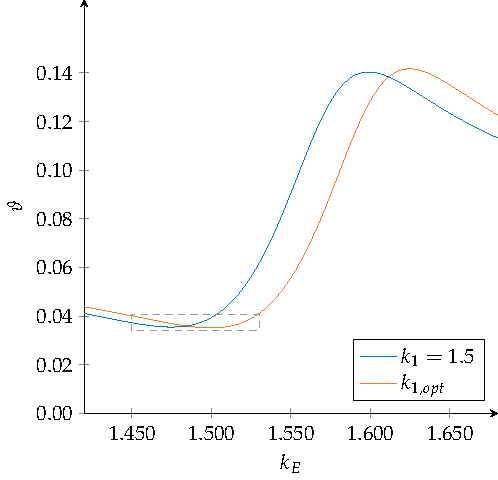
\includegraphics[page=1,width=0.45\textwidth]{TikzNurkoptGanzBereich}}
	\hfill
	\subcaptionbox{Vergrößerte Darstellung des in \figref{fig:Opt:Beispiel:Optimalesk1GanzerBereich} grau gestrichelt gekennzeichneten Bereichs. Durch die Wahl von $k_{1,opt}$ statt $k_1=1.5$ ergibt sich eine Performanceverbesserung von $\D \vartheta = 12.1\%$ an der Stelle $k_E=1.5$
	\label{fig:Opt:Beispiel:Optimalesk1GanzerZoom}}% 
	[0.48\linewidth]{\includegraphics[page=2,width=0.45\textwidth]{TikzNurkoptGanzBereich}}
	
	\caption[Verlauf der Drehungleichförmigkeit als Funktion der Anregungsordnung]{Verlauf der Drehungleichförmigkeit $\vartheta$ für $k_1=1.5$ und $k_{1,opt} = 1.525$ als Funktion der Anregungsordnung $k_E$ mit $\Gamma = \nicefrac{1}{10}$,  $\epsilon = \nicefrac{1}{10}$,  $\delta_1 = 1$}
	\label{fig:Opt:Beispiel:Optimalesk1UeberkE}
\end{figure}
%
%
%
Im hier betrachteten Beispiel soll für ein Standardpendel ohne Mistuning ($u_{1,2}=0$) $\vartheta$ bei $k_E=1.5$ minimal werden. 
Mit den Startwerten $k_{1,0}=1.5$, $I_{a1,0}=2.9 \cdot 10^{-3}$ und $\theta_{a1,0}= 1.3$ für 
$\Gamma = \nicefrac{1}{10}$,  $\epsilon = \nicefrac{1}{10}$ und  $\delta_1 = 1$ ergibt sich das optimale Tuning zu $k_{1,opt} = 1.525$. In \figref{fig:Opt:Beispiel:Optimalesk1UeberkE}  ist
der resultierende Verlauf der Drehungleichförmigkeit $\vartheta$ über der Anregungsordnung $k_E$ für $k_{1,opt} = 1.525$ im
Vergleich zum Verlauf für $k_1 =1.5$  dargestellt. 
Es lässt sich deutlich erkennen, dass das Minimum für den Verlauf mit $k_{1,opt} = 1.525$ 
 bei $k_E = 1.5$ liegt. 
%
Die Wahl von $k_{1,opt}=1.525$ statt $k_1=1.5$ führt dazu, dass sich das Minimum des Verlaufs von $\vartheta$ um
$\D k_E=0.025$ von der Anregungsordnung $k_{E,shift} = 1.475$ zur gewünschten Anregungsordnung $k_E=1.5$ verschiebt.
Mit den hier gewählten Parametern ergibt sich dadurch eine Performanceverbesserung 
von $\D \vartheta = 12.1\%$.
%
Ein mit $k_{1,opt}$ getunter Absorber zeigt  im Gegensatz zu einem mit $k_1 = k_E$ getunten Absorber 
bei der Anregungsordnung $k_E$ eine deutlich bessere Schwingungsreduktionswirkung. 
Allgemein lässt sich auf Basis der hergeleiteten Minimumsbedingung 
immer das optimale Tuning $k_1$ für eine bestimmte Anregungsordnung $k_E$ berechnen,
um dann genau bei dieser Anregungsordnung bestmögliche Performance des Absorbers zu erzielen. 	

%
%
%
%
%
\begin{figure}[ht]%
	\centering
	\subcaptionbox{Verlauf der Drehungleichförmigkeit $\vartheta$ für $k_1=1.5$ und $k_{1,opt} = 1.525$ 
		als Funktion der Anregungsamplitude $\Gamma$ \label{fig:Opt:Beispiel:Optimalesk1UeberGammaDrehunGl}}
	[0.48\textwidth]{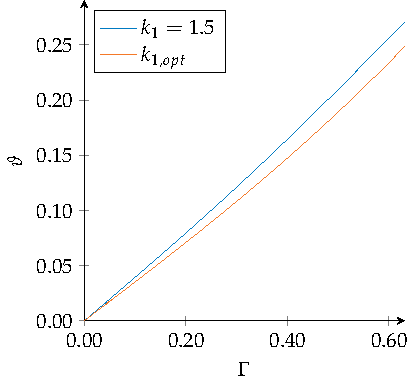
\includegraphics{TikzNurkopt}}
	\hfill
	\subcaptionbox{Prozentuale Performanceverbesserung $\D \vartheta$ des mit $k_{1,opt} = 1.525$  getunten Absorbers gegenüber dem mit $k_1=1.5$ getunten Absorbers \label{fig:Opt:Beispiel:Optimalesk1UeberGammaInProzent}}
	[0.48\textwidth]{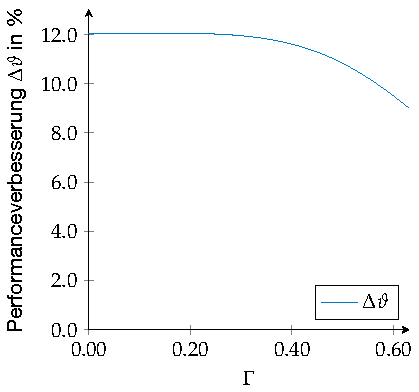
\includegraphics{Vergleichk1Undk1optUeberGammaInProzent-7-7}}
	
	\caption[Verlauf der Drehungleichförmigkeit als Funktion der Anregungsamplitude]{Verlauf der Drehungleichförmigkeit $\vartheta$ für $k_1=1.5$ und $k_{1,opt} = 1.525$ 
				als Funktion der Anregungsamplitude $\Gamma$ mit $k_E = 1.5$,  $\epsilon = \nicefrac{1}{10}$,  $\delta_1 = 1$
				und prozentuale Verbesserung der Performance $\D \vartheta$}
	\label{fig:Opt:Beispiel:Optimalesk1UeberGamma}
\end{figure}
%
%
%
%
%
%
%
\figref{fig:Opt:Beispiel:Optimalesk1UeberGammaDrehunGl} zeigt darüber hinaus, dass die Drehungleichförmigkeit $\vartheta$ für $k_{1,opt} = 1.525$ bei Anregungsordnung $k_E=1.5$ auch
für veränderliche Anregungsamplituden  $\Gamma$  immer kleinere Werte als ein mit $k_1$ getunter Absorber annimmt. 
Der Absorber mit optimalem Tuning $k_{1,opt}$ zeigt bei allen Anregungsamplituden 
bessere Performance als ein mit $k_1=k_E$ getunter Absorber.
In \figref{fig:Opt:Beispiel:Optimalesk1UeberGammaInProzent} ist zur Veranschaulichung
die prozentuale Performanceverbesserung $\D \vartheta$ in Abhängigkeit der
Anregungsamplitude  $\Gamma$ für die verwendeten Parameter dargestellt.


Die beschriebene Optimierung beschränkt sich nicht rein auf die Wahl eines optimalen Tunings $k_1$. 
Ebenso könnten die Parameter im nichtlinearen Mistuning $u_1(s_1)$, wie in den Gleichungen in  \secref{Opt:Bsp:AveragingGleichungen} berücksichtigt, optimiert werden.
Wird beispielsweise $u_1$ als Polynom angesetzt, stellen die Koeffizienten dieses Polynoms weitere Optimierungsparameter dar. 
Beispielsweise tritt für einen Mistuning-Ansatz nach Gleichung 	\eqref{eq:Opt:Bsp:MistAnsatz2terOrdn} in den im 
Optimierungsproblem als Gleichungsnebenbedingungen berücksichtigten Averaging-Gleichungen 	\eqref{eq:OptBspGleichungThetaa1} und \eqref{eq:OptBspGleichungIa1} ein Zusatzterm
durch den Koeffizient $u_{1,2}$ auf und die Zielfunktion $\vartheta$ ist als $\vartheta = \vartheta(k_1,I_{a1},\theta_{a1}, u_{1,2}) $ anzusetzen.
Dies ist bei der Implementierung bereits berücksichtigt.
Eine Erweiterung durch weitere Terme in $u_1(s_1)$ erfolgt analog.
Anderenfalls könnte aber auch von vornherein ein beliebiger Zusammenhang für $u_1(s_1)$ gegeben sein,   
womit wie im dargestellten Beispiel nur $k_{1,opt}$ zu bestimmen ist.  
Dann werden ebenfalls die Averaging-Gleichungen durch die aus dem Mistuning 
resultierenden Terme erweitert, aber die Zielfunktion $\vartheta = \vartheta(k_1,I_{a1},\theta_{a1})$ 
bleibt davon unbeeinflusst.




Zusammenfassend lässt sich festhalten, dass durch die hergeleitete Minimumsbedingung eine Bestimmung des optimalen Tunings $k_1$ möglich ist, jedoch
auch weitere Parameter in den Optimierungsprozess ohne großen Aufwand mit aufgenommen werden können. 









%\newpage
%
%
% SUBOPTIMALES TUNING
%
\subsubsection{Suboptimales Tuning \texorpdfstring{$k_{1,subopt}$}{k1subopt} }

Zu Beginn dieses Abschnitts wurde darauf hingewiesen, dass die Startwerte für $k_1$, $I_{a1}$ und $\theta_{a1}$ im betrachteten Beispiel in der Nähe der erwarteten Lösung zu wählen sind. 
Außerdem wurde gegen Ende von \secref{Opt:Theorie:BestDerGrad} angemerkt, dass es sich bei der Minimumsbedingung \eqref{eq:OptMinimumsbedinungEndg} 
um eine notwendige Bedingung handelt und im Fall, dass Gleichung	\eqref{eq:OptMinimumsbedinungEndg} erfüllt ist bzw.  mehrere Lösungen besitzt, 
die potentiellen Lösungen noch darauf zu prüfen sind, ob ein Minimum vorliegt.
Dies soll zu Abschluss dieses Kapitels genauer betrachtet werden.

Wird die Optimierung mit den (konstruierten) Startwerten $k_{1,0}=1.1$, $I_{a1,0}=7.3 \cdot 10^{-3}$ und $\theta_{a1,0}= 0.05$ bei sonst identischen Parametern  initialisiert, berechnet sich 
das zunächst als optimal erwartete Tuning zu $k_{1,subopt} = 1.405$. 	
%
%
\begin{figure}[bt]%
	\centering
	\begin{subfigure}{0.49\textwidth}
	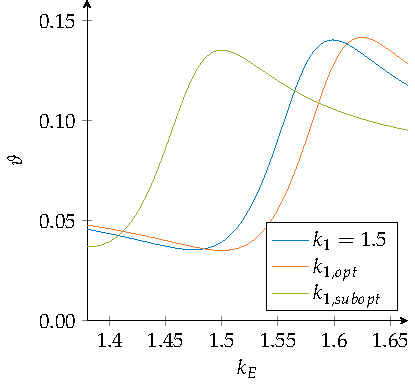
\includegraphics{TikzAuchksubopt-kE} \label{fig:Opt:Beispiel:VerlaufVonVarthetaFuerSuboptimalesk1UeberkE}
	\caption{Verlauf von $\vartheta$ als Funktion der Anregungsordnung $k_E$ für $\Gamma = \nicefrac{1}{10}$}
	\end{subfigure}
	\hfill
	\begin{subfigure}{0.49\textwidth}
	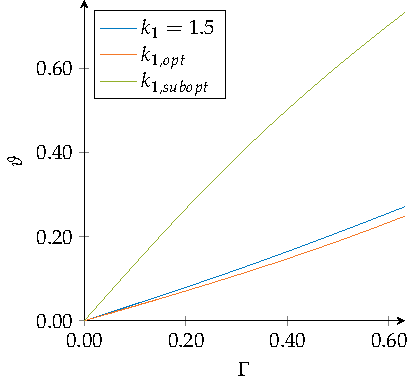
\includegraphics{TikzAuchksubopt-Gamma} \label{fig:Opt:Beispiel:VerlaufVonVarthetaFuerSuboptimalesk1UeberGamma}
	\caption{Verlauf von $\vartheta$ als Funktion der Anregungsamplitude $\Gamma$ für $k_E = 1.5$}
	\end{subfigure}

	\caption[Verlauf der Drehungleichförmigkeit $\vartheta$ für $k_1=1.5$, $k_{1,opt} = 1.525$]
					{Verlauf der Drehungleichförmigkeit $\vartheta$ für $k_1=1.5$, $k_{1,opt} = 1.525$ und $k_{1,subopt}=1.405$ 
					mit $\epsilon = \nicefrac{1}{10}$,  $\delta_1 = 1$;
					$k_{1,opt}$ ist so gewählt, dass das Minimum des Verlaufs von $\vartheta$ bei $k_E=1.5$ liegt; 
					$k_{1,subopt}$ hingegen ist so gewählt, dass das Maximums des Verlaufs von $\vartheta$ bei $k_E=1.5$ liegt	}
	\label{fig:Opt:Beispiel:VerlaufVonVarthetaFuerSuboptimalesk1}
\end{figure}
%
%
%
\figref{fig:Opt:Beispiel:VerlaufVonVarthetaFuerSuboptimalesk1} zeigt die aus 	\figref{fig:Opt:Beispiel:Optimalesk1UeberkE} 
und	\figref{fig:Opt:Beispiel:Optimalesk1UeberGamma} bekannten Graphen mit den für $k_{1,subopt}=1.405$  erweiterten
Verläufen für die Drehungleichförmigkeit $\vartheta$. 
Ein Tuning von $k_{1,subopt}=1.405$ führt im betrachteten Fall dazu, dass sich das Maximum  (und nicht das Minimum)
von $\vartheta$ an der Stelle $k_E=1.5$ befindet (siehe \figref{fig:Opt:Beispiel:VerlaufVonVarthetaFuerSuboptimalesk1UeberkE}), 
was der schlecht möglichsten Absorberperformance an dieser Stelle gleich kommt. Eine extreme Verschlechterung resultiert auch bei
veränderlicher Anregungsamplitude  $\Gamma$ %an allen Stellen 
(vgl. \figref{fig:Opt:Beispiel:VerlaufVonVarthetaFuerSuboptimalesk1UeberGamma}).

Dieses Beispiel verdeutlicht, dass durch die notwendige Bedingung \eqref{eq:OptMinimumsbedinungEndg} bei Initialisierung mit
ungünstigen Anfangswerten auch eine
Lösung für das Tuning berechnet werden kann, welche ein Maximum  von $\vartheta$ an einer bestimmten Stelle $k_E$ zur Folge hat.
Um dies zu vermeiden, ist es von großer Bedeutung die Optimierung mit sinnvollen Anfangswerten zu initialisieren (vgl. Anmerkungen zu Beginn dieses
Abschnitts) und im Anschluss daran zu prüfen, ob wirklich das optimale Tuning berechnet wurde.

